\documentclass[a4paper, 11pt]{article}
\usepackage[left=2cm, top=3cm, text={17cm, 24cm} ]{geometry}
\usepackage[utf8]{inputenc}
\usepackage[czech]{babel}
\usepackage{times}
\usepackage[unicode, hidelinks]{hyperref}
\usepackage{graphicx}
\usepackage{minted}


\graphicspath{{./img/}}

\begin{document}

\begin{titlepage}
    \begin{center}
        
\includegraphics[scale=0.15]{fit_logo.png}\\
        \vspace{\stretch{0.39}} \\
        \huge ISS Projekt 2021/2022 \\ 
        \hfill \break
        \huge Jakub Kuzník \\
        \huge xkuzni04 \\

        \vspace{\stretch{0.61}}
        {\Large\noindent \today}
    \end{center}
    
\end{titlepage}

\tableofcontents
\newpage



%
% ZÁKLADY ##############################################
\section{Základy}
    Pro uložení signálu a vzorkovací frekvence jsem použil funkce knihovny scipy.io.
    \begin{minted}{python}
        sample_rate, data = wavfile.read(filepath)
    \end{minted}  
    \\
Celkový čas signálu jsem zjistil pomocí vzorkovací frekvence a počtu vzorků. Data jsem poté zpracoval pomocí následující funkce.  

\begin{minted}{python}

    def basic_signal_info(data, sample_rate):

        data_min = data.min()
        data_max = data.max()
        lenght_sec = (data.shape[0] / sample_rate)
        lenght_sam = data.shape[0]

        return data_min, data_max, lenght_sec, lenght_sam
\end{minted} \\\\

Data, která jsem zjistil: \\

\begin{table}[ht]
		\centering
		\begin{tabular}{| c | c | c |}
			\hline
			Veličina & \small Hodnota & \small Jednotky &
			\hline
	Vzorkovací frekvence & 16000 &  vzorků/s \begin{tabular}{l}  \end{tabular} \\
			\small Časová délka signálu & 1.9968125 & s  \begin{tabular}{l}  \end{tabular} \\
			\small Délka signálu ve vzorcích & 31949 &   vzorků  \begin{tabular}{l}  \end{tabular} \\
			\small Maximální hodnota  & 12518 &  \begin{tabular}{l}  \end{tabular} \\
			\small Minimální hodnota  & -9448 &    \begin{tabular}{l}  \end{tabular} \\ \hline

		\end{tabular}
		\label{table:rozdeleni_prace}
\end{table}

Signál jsem poté vykreslil pomocí funkce \texttt{plt} a tohle je výsledná podoba. Pro časovou osu jsem zvolil čas od začátku signálu do konce.
\begin{center}
\end{center}
    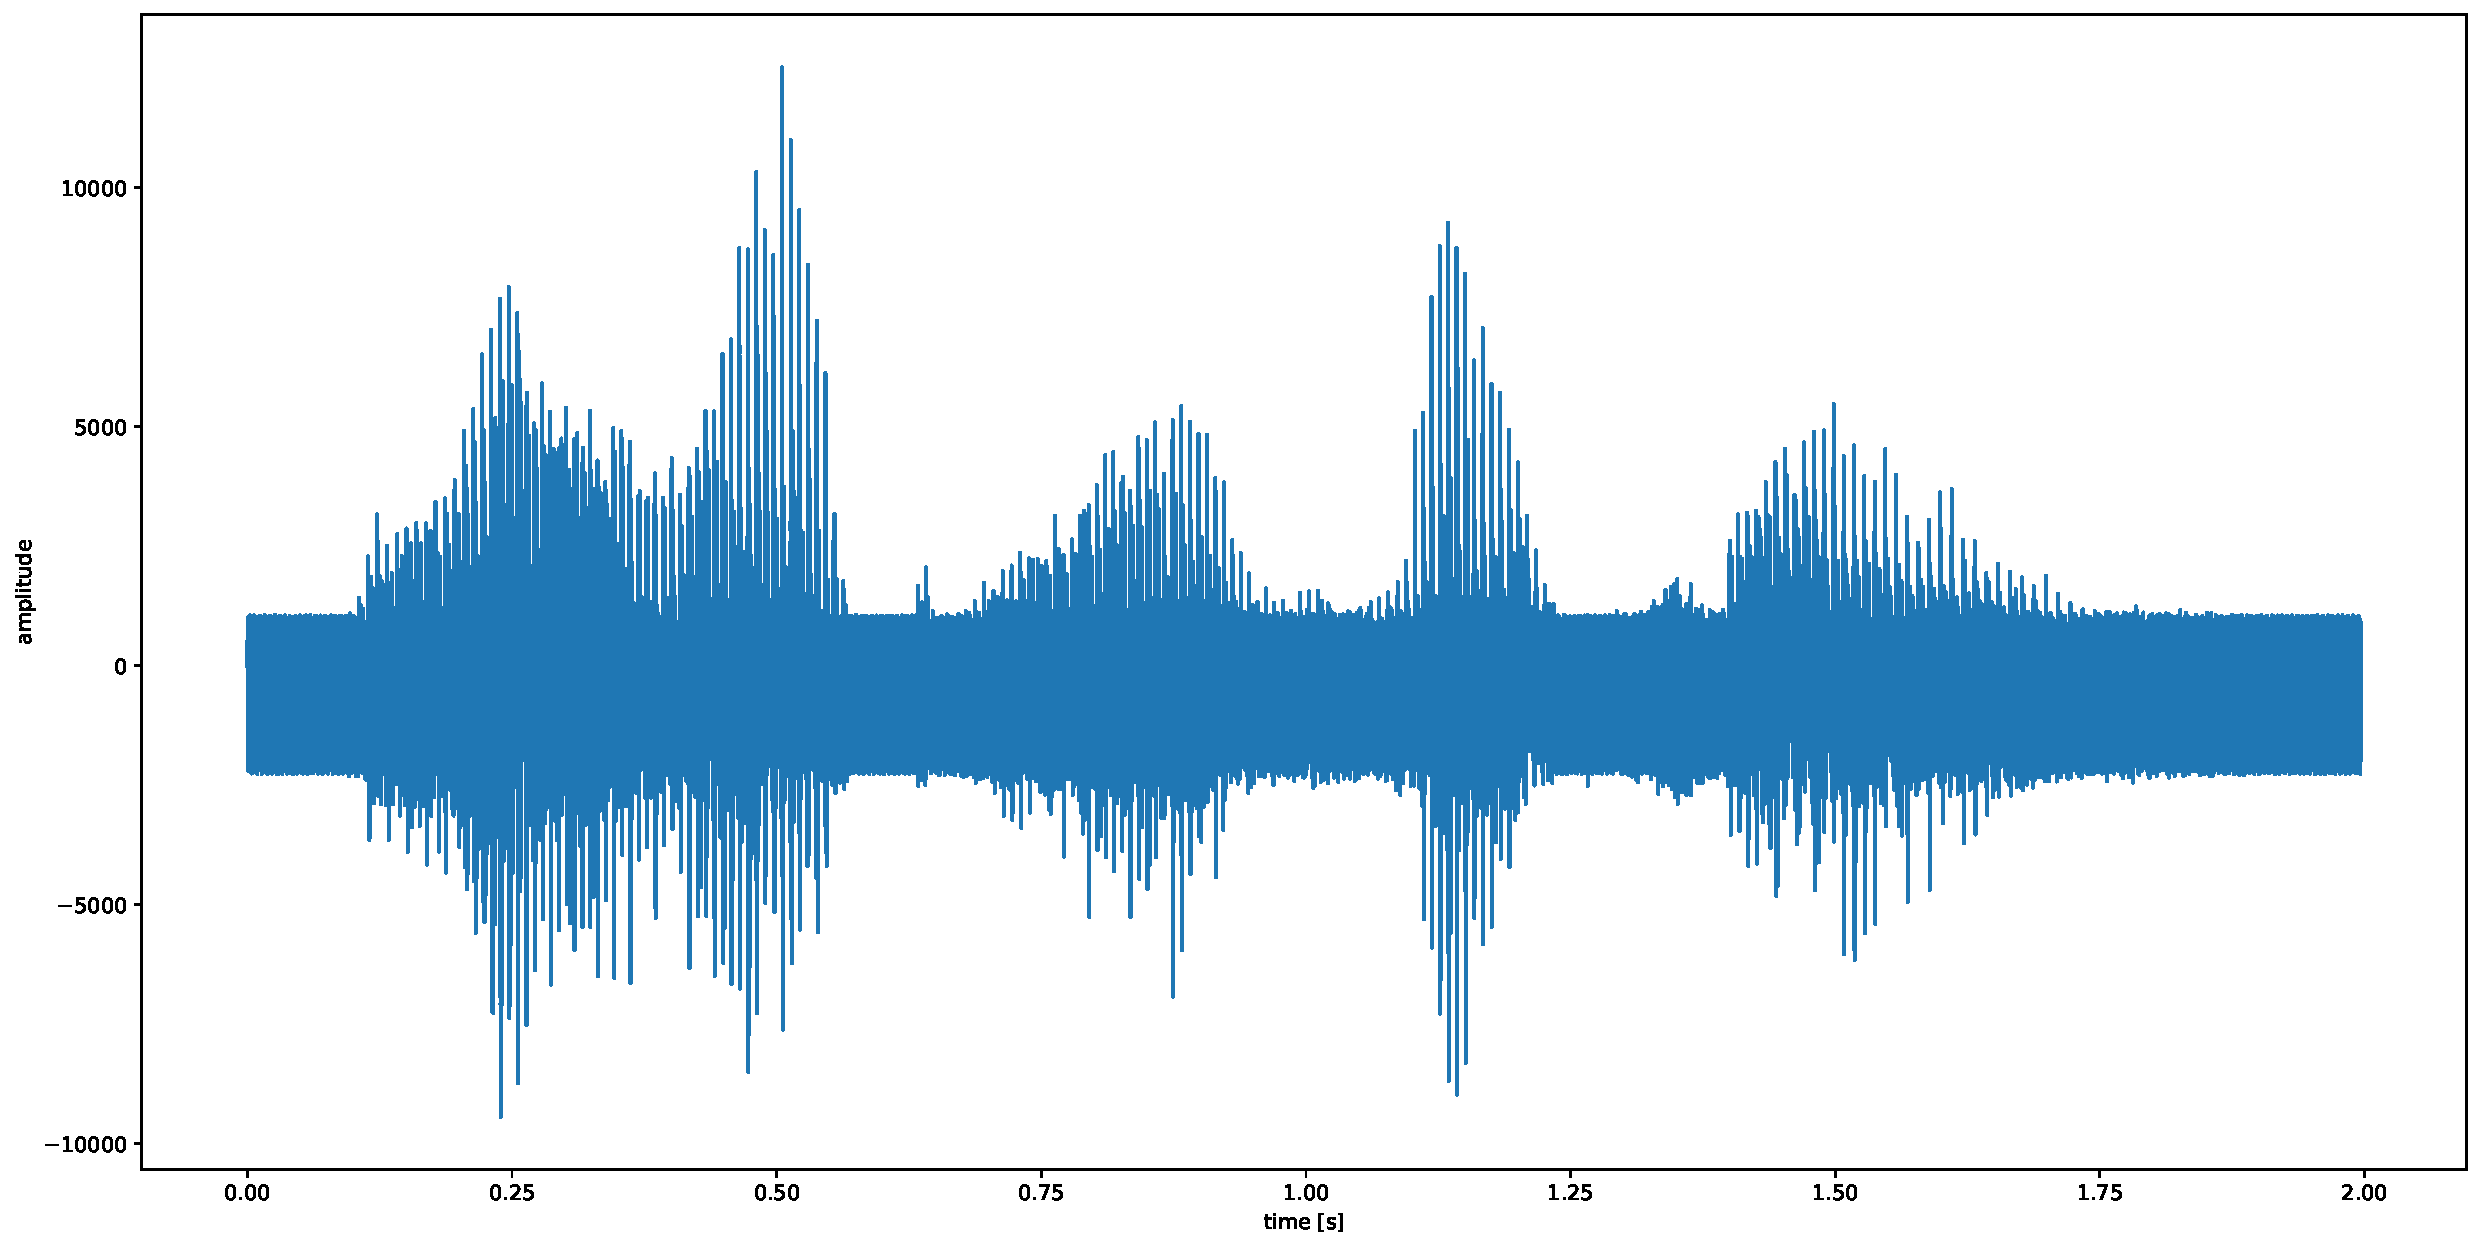
\includegraphics[scale=0.4]{img/0_input_signal.pdf}
% ####################################################




%
% Předzpracování a rámce ##############################################
\section{Předzpracování a rámce}
% ####################################################
    Signál jsem prvně vycentroval a normalizoval, tedy změnil rozsah hodnot na (-1,1) a od každého vzorku odečetl střední hodnotu.
     \begin{minted}{python}
        #Centrování 
        data = data - mean(data) #mean je funkce pro výpočet střední hodnoty
        
        # normalizace dat 
        data_abs = abs(data)
        max_value = max(data_abs)
        return (data / max_value) 

    \end{minted}
    Následně jsem tato data pomocí vektorového for cyklu zpracoval do rámců o délce 1024 s překrytím 512. To mi dalo délku rámce rovnou 0.064s.
    \begin{minted}{python}
        inc = 512       # překrytí o 512 vzorků
        width = 1024    # délka jednoho rámce       
        new_data = []   # proměnná pro nová data 
    
        for i in range(0, lenght_sam, inc):
            new_data += [data[i:i+width]]

        new_data = np.array(new_data) ## ještě je potřeba transponovat matici
    \end{minted}
    Na obrázku už mám jeden vykreslený rámec - konkrétně se jedná o rámec s indexem číslo 10 neboli 11. rámec. U něj jsem jenom musel dopočítat odpovídající čas, to jsem udělal pomocí vzorkovací frekvence. Takže čas na ose x reálně odpovídá tomu, kde v signálu se tento rámec nachází.\\ 
    
    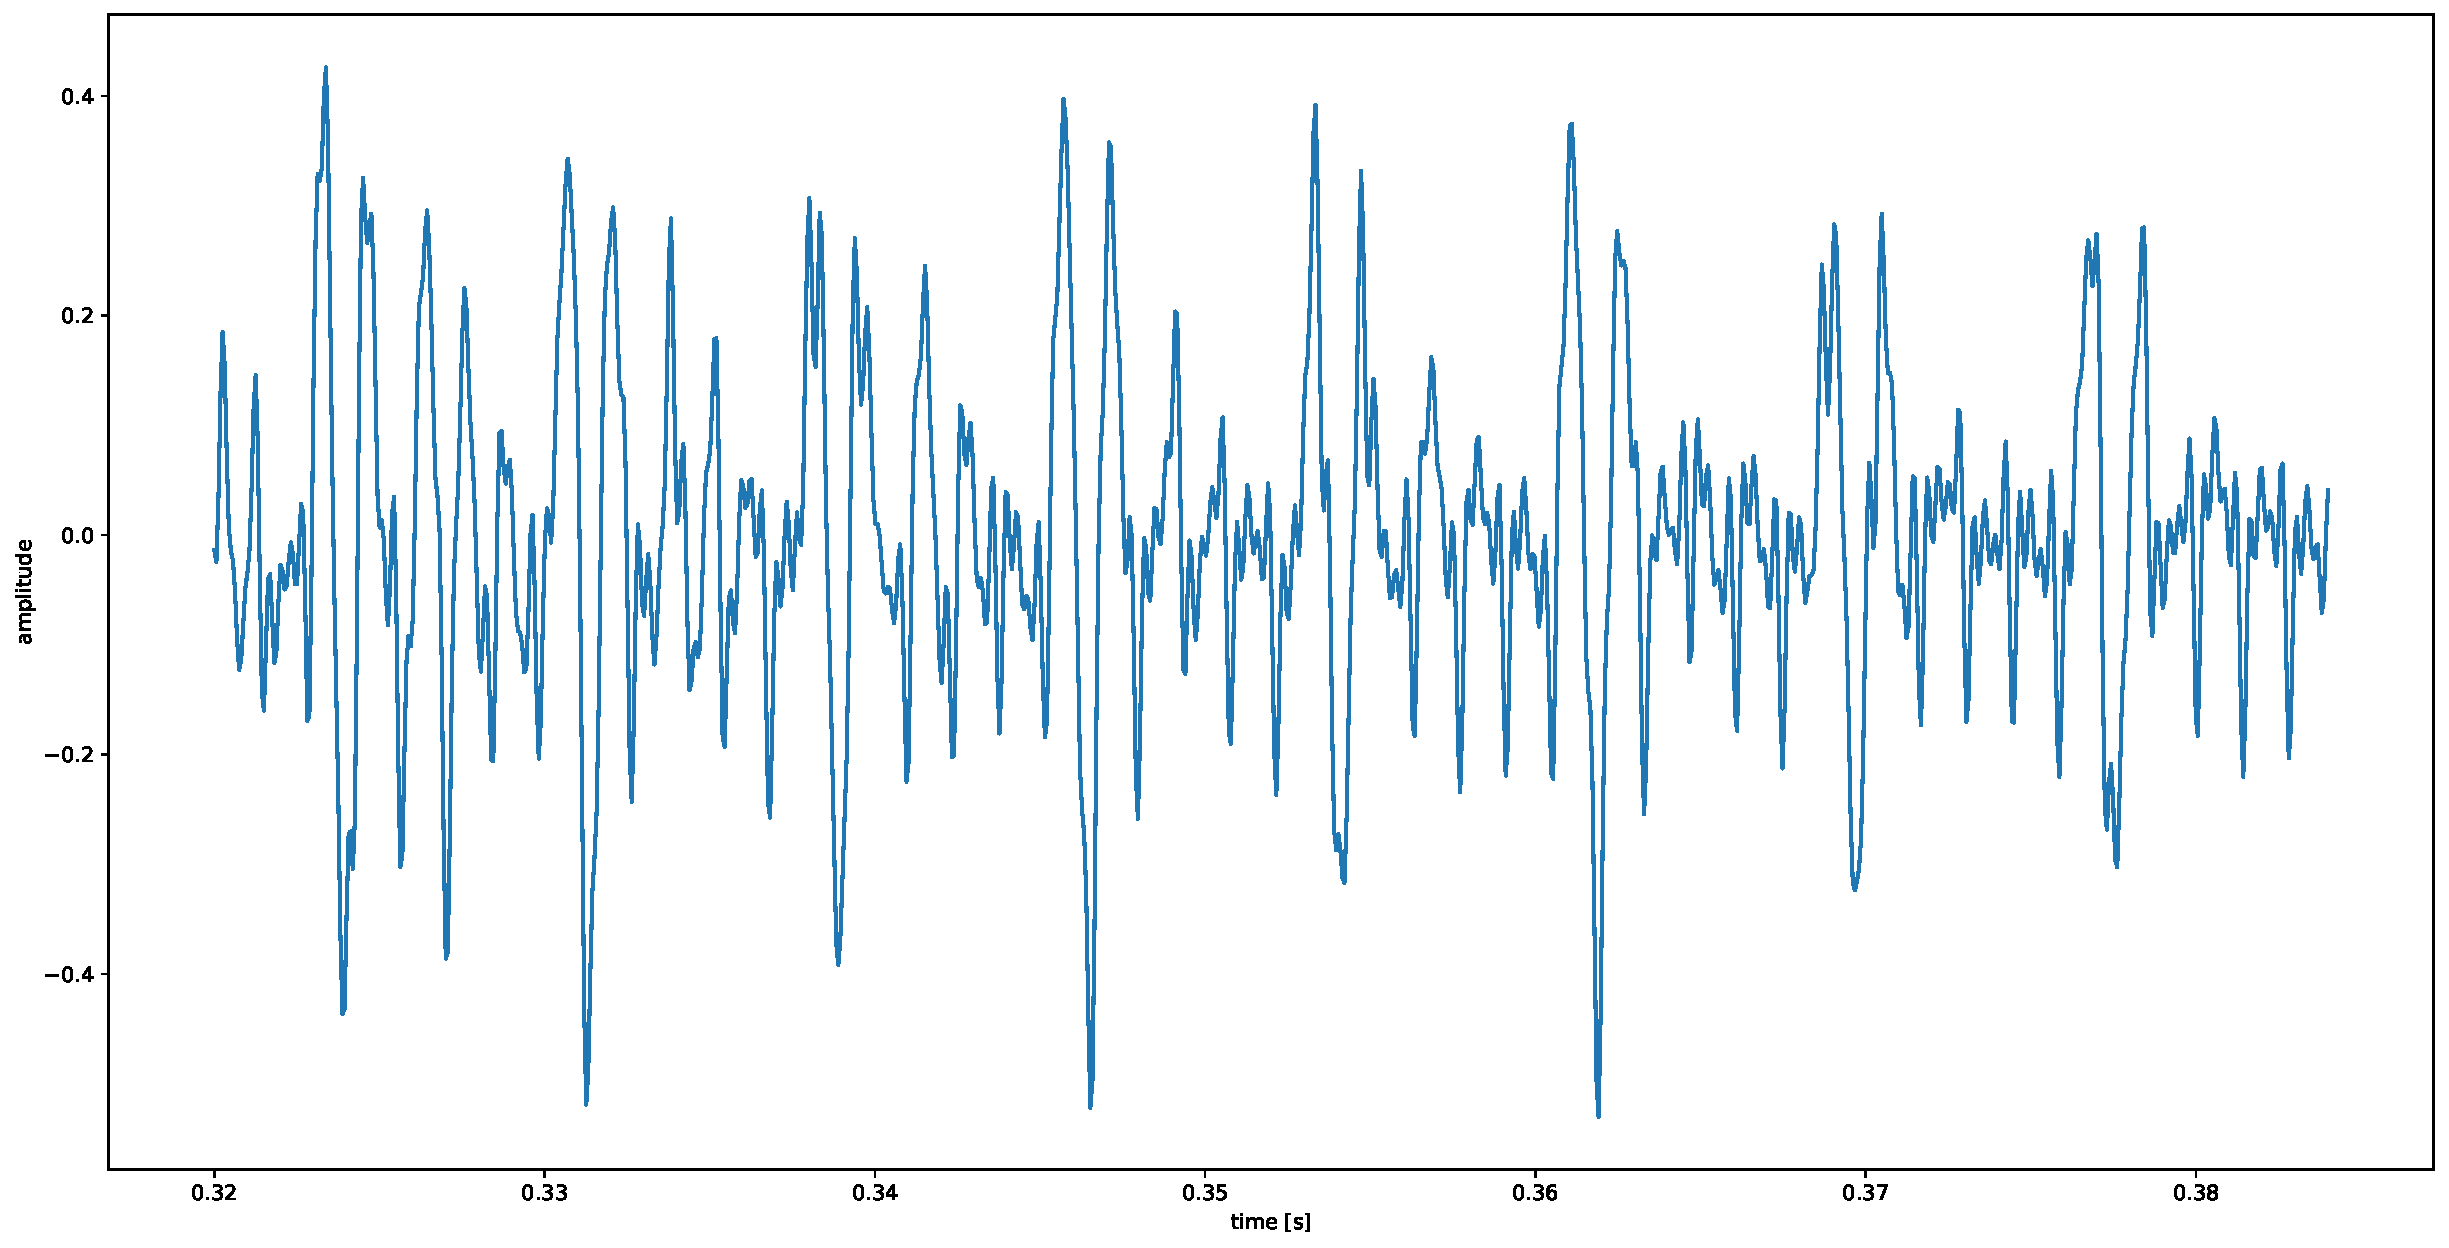
\includegraphics[scale=0.4]{img/1_frame2.pdf}


% DFT ##############################################
\newpage
\section{DFT}
% ####################################################
Moje DFT je vytvořená pro stejný rámec, jako byl zobrazen v předchozí úloze, ale hodnoty jsou zobrazeny jenom do poloviny rámce - poté totiž začala být funkce osově souměrná.\\

\begin{minted}{python}
##
# Funkce pro realizaci DFT na jeden rámec
def dtf_func(data, index):
    
    one_frame = data[index] # v datech mám uloženy všechny rámce 
    
    N = len(one_frame)      # počet vzorků rámce
    # jelikož je DFT symetrické pracuji jenom s polovinou rámce
    half = math.ceil(N/2)  

    n = np.arange(N)        # Vytvoří hodnoty od 0 po počet N
    k = n.reshape((N, 1))   # transformace matice 
    M = np.exp(-2j * np.pi * k * n / N) # vzorec DFT
    fourier = np.dot(M, one_frame) 
    return np.abs(fourier[0:half]) # vratím hodnoty od 0 po half
\end{minted}

Zde je výsledek DFT jednoho znělého rámce. Na ose x jde vidět, že i když je délka rámce 1024, vykresluji jenom 512 hodnot. \\

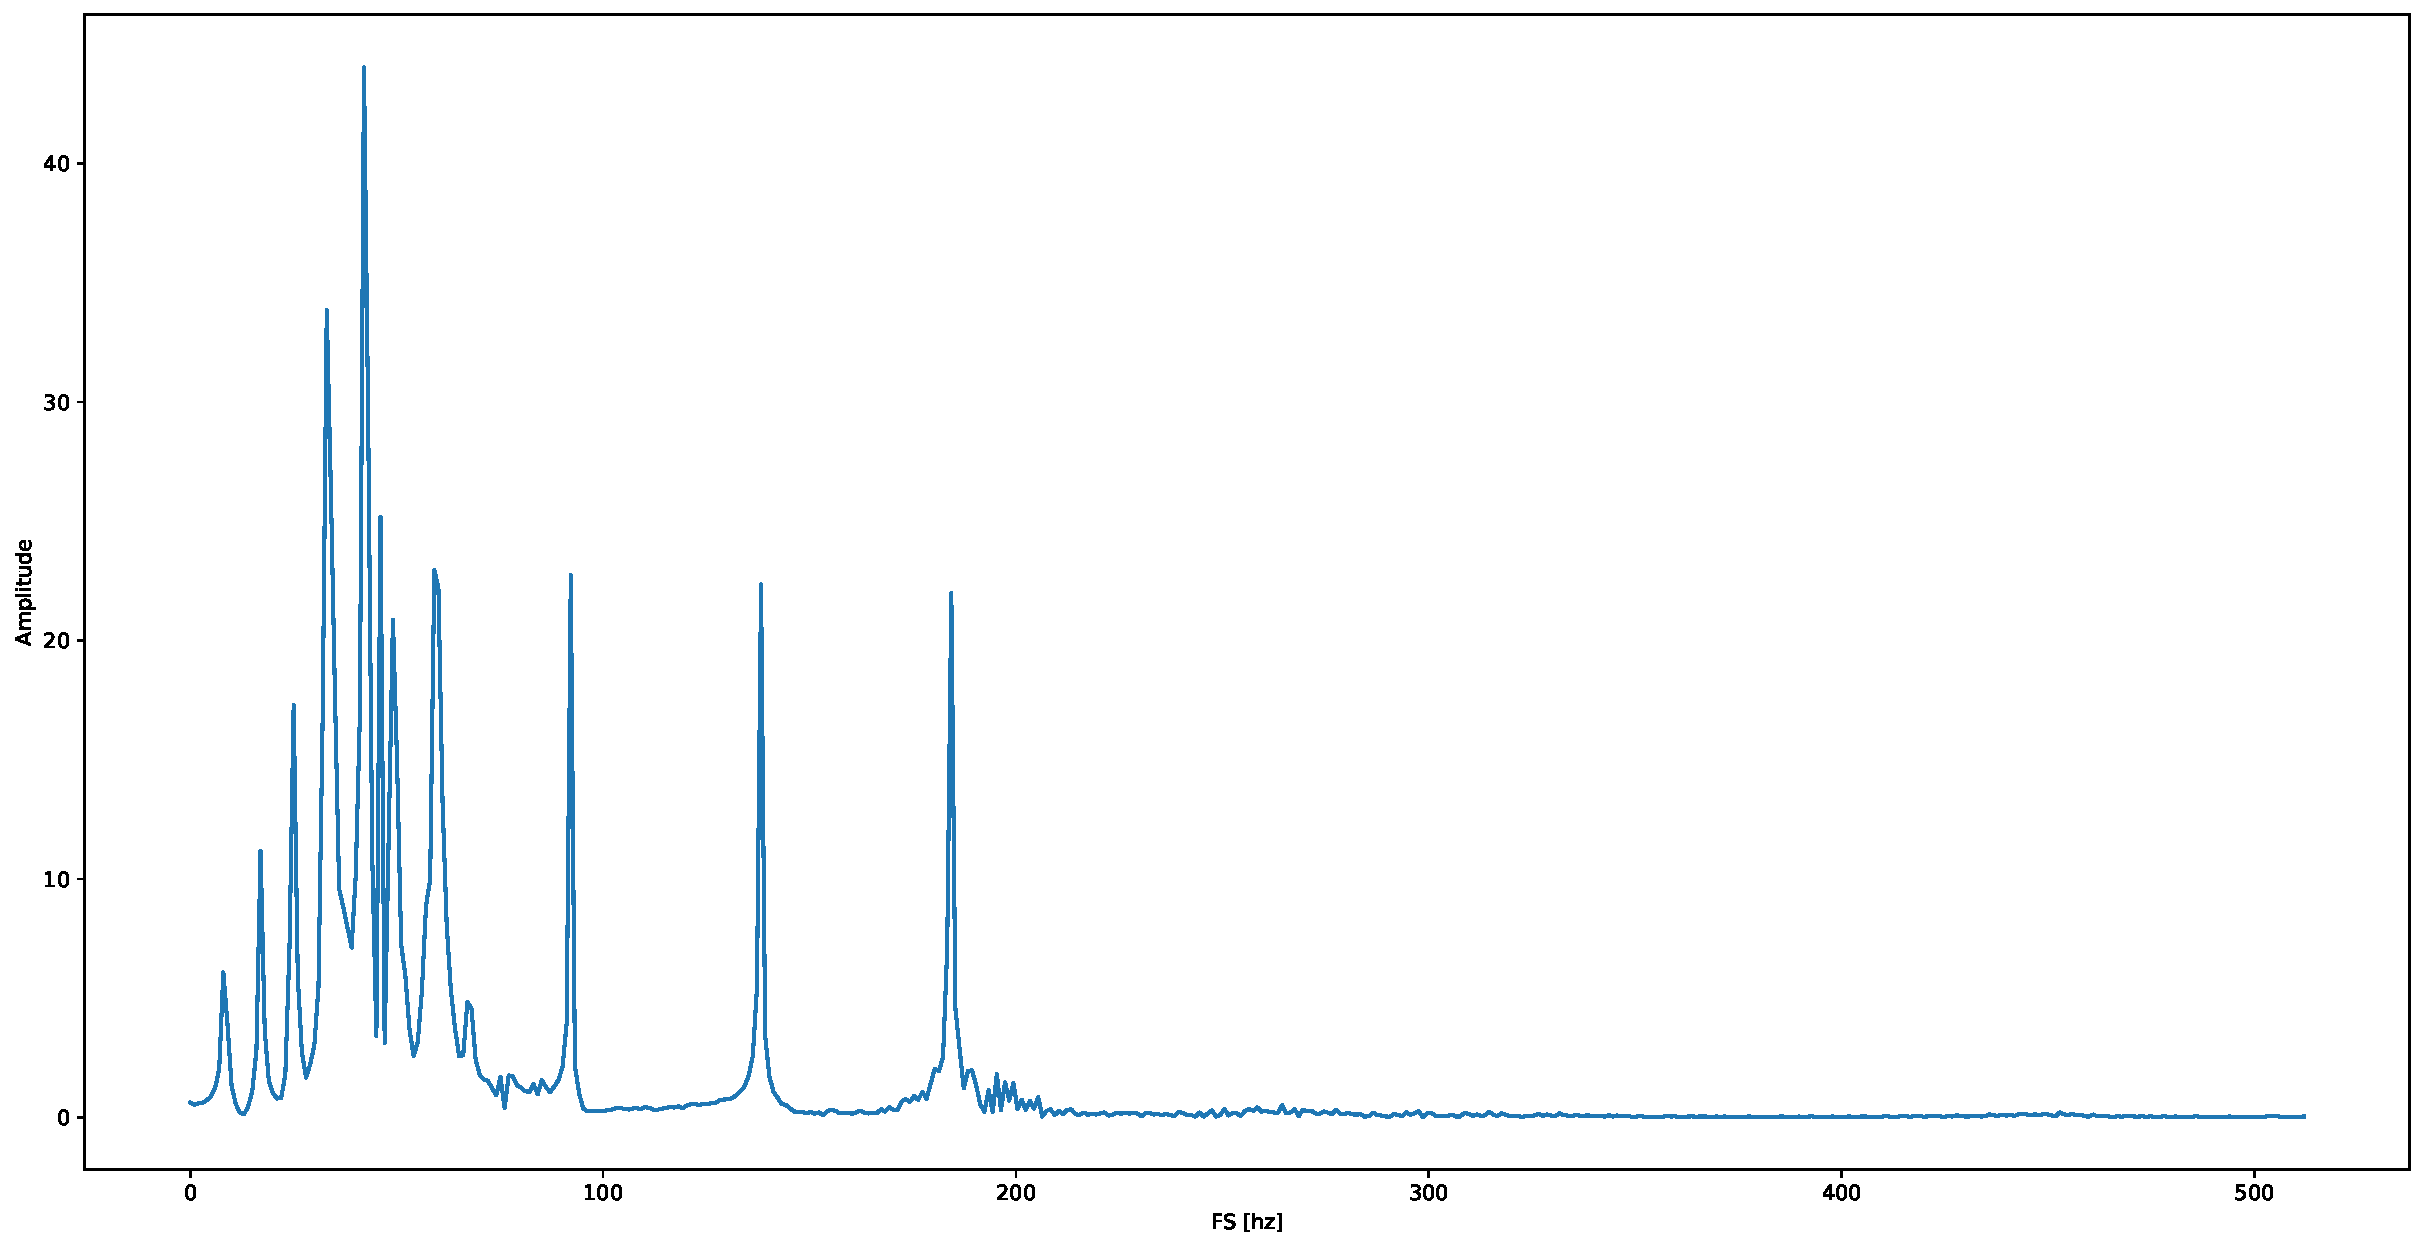
\includegraphics[scale=0.38]{img/2_dft.pdf} \\


% Určení rušivých frekvencí ##############################################
\newpage 
\section{Spektrogram}
Zde je můj spektrogram ukazující frekvence jednotlivých koeficientů DFT. Ze spektrogramu se dá vyčíst, jak moc se jednotlivé frekvence vyskytují v signále, a to v čase, který je reprezentován osou x. Na první pohled je vidět, že se zde vyskytují 4 podivné horizontální čáry žluté barvy, zhruba kolem frekvence 800Hz, 1400Hz, 2100Hz a 2900Hz \\ 

\begin{minted}{python}
    # Data jsou v čisté podobě pouze normalizovaná a vycentrovaná 
    data = center_signal(data)
    data = normalize_signal(data)
    
    frame_width = 1024 # Velikost jednoho rámce
    noverlap = 512     # Překrytí rámců. 

    #Zde jsem použil funkci knihovny matplotlib.pyplot
    plt.specgram(data, Fs=sample_rate, NFFT=frame_width, \\
                 noverlap=noverlap, mode='psd', scale='dB')

\end{minted}

A tohle už je výsledek implementace. \\
\begin{center}
    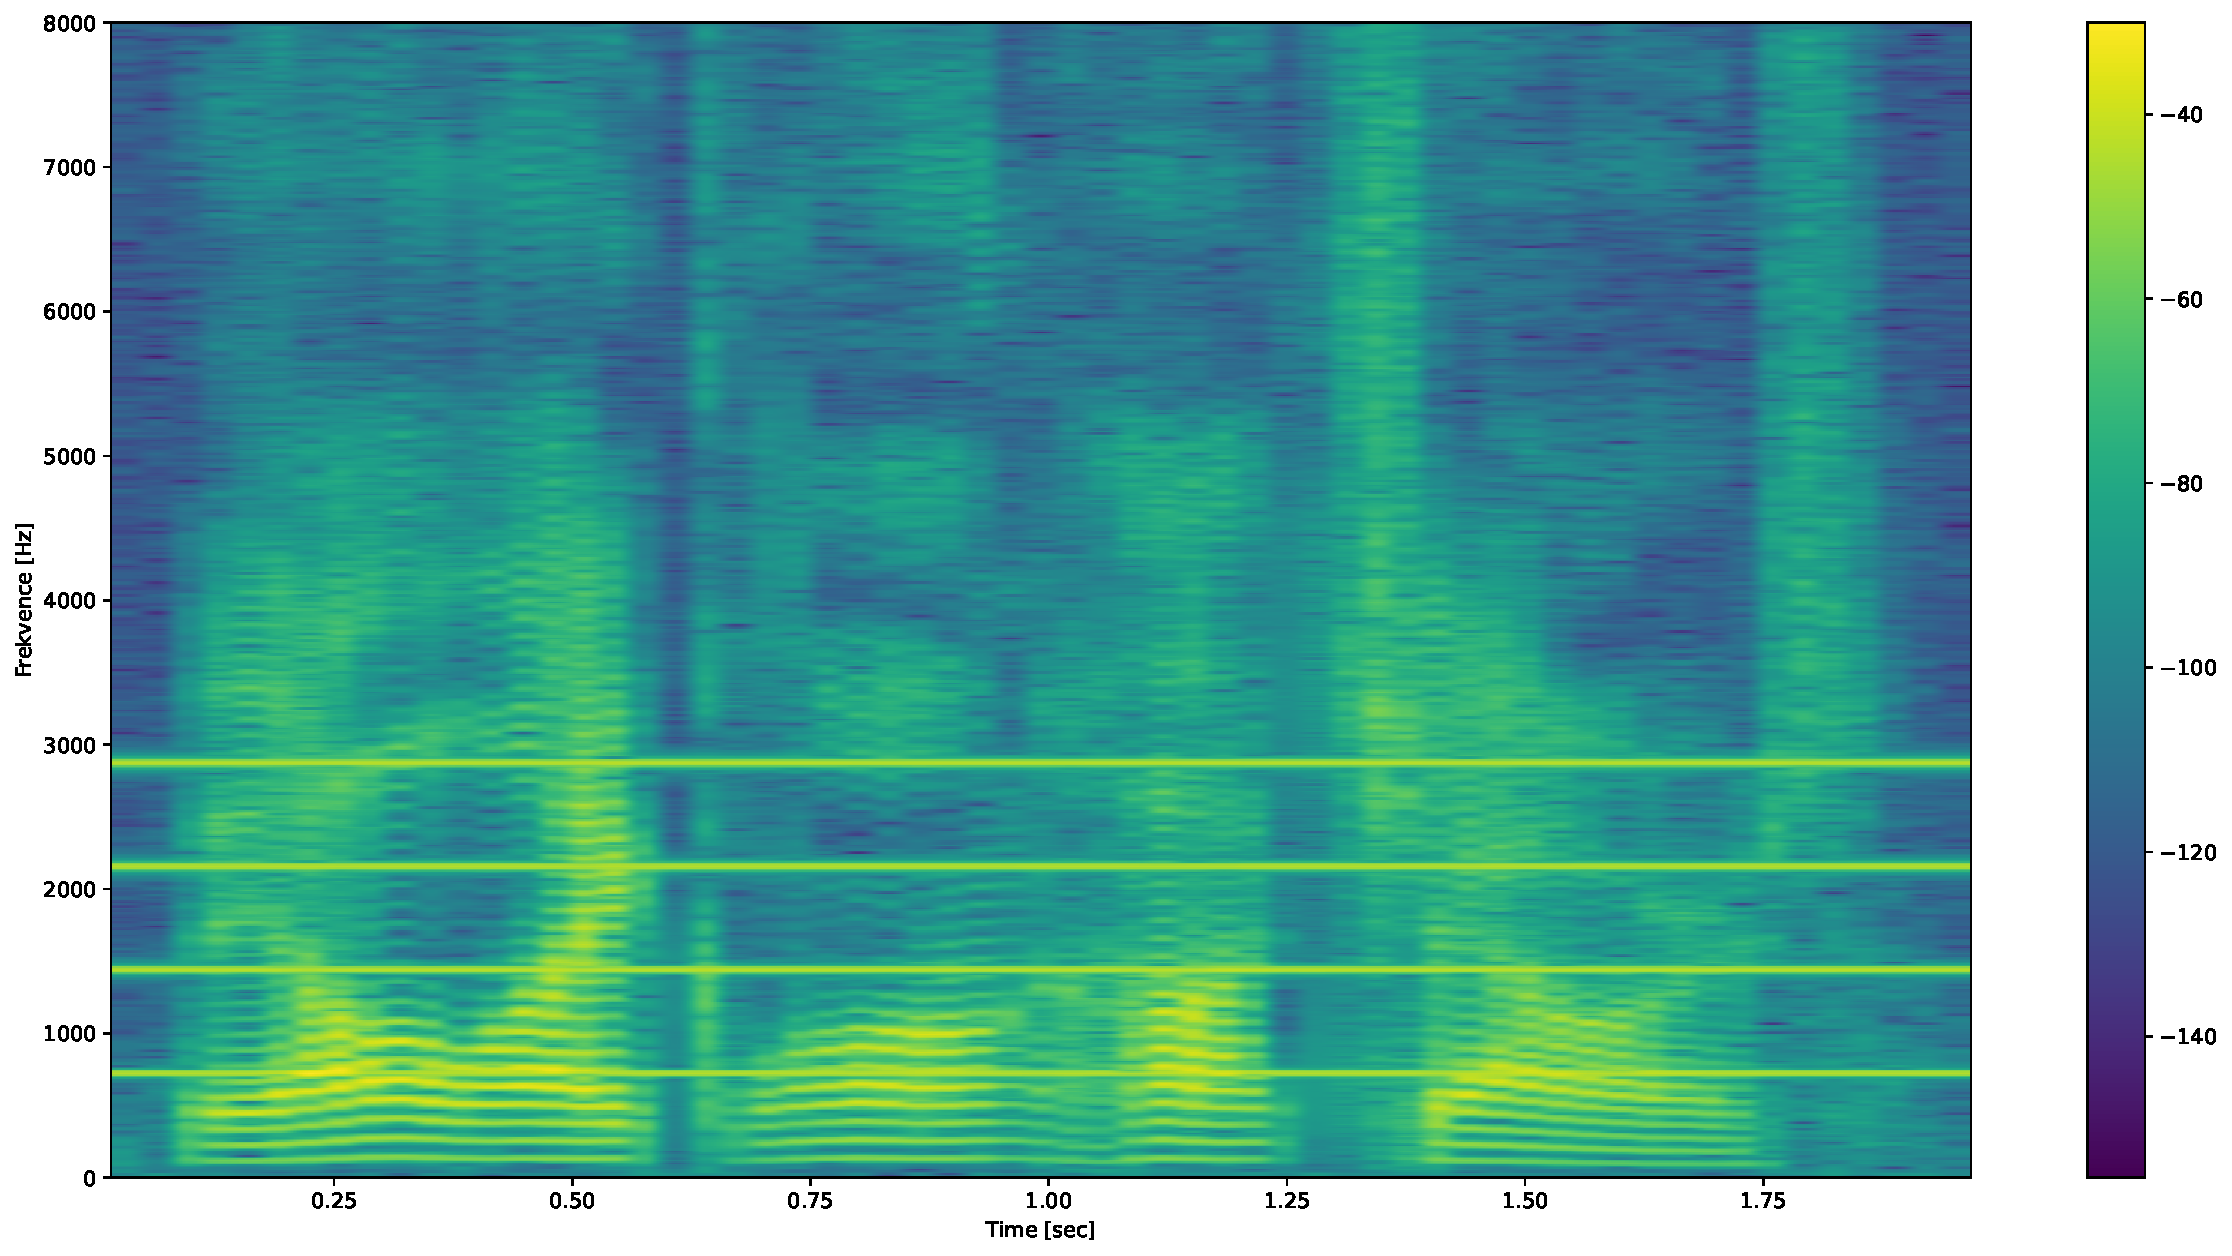
\includegraphics[scale=0.35]{img/3_spec.pdf} \\
\end{center}
 
\\

% ####################################################


% Určení rušivých frekvencí ##############################################
\section{Určení rušivých frekvencí}

Z spektrogramu jsem vyčetl následující rušivé frekvence. Na první pohled jde vidět, že hodnoty jsou násobkem první rušivé frekvence f1, jelikož   f2 = f1*2 a    f3 = f1*3    atd. 

\begin{table}[ht]
    \centering
    \begin{tabular}{| c | c |}
    \hline
        Rušivý signál & Frekvence [Hz]  \\ \hline
        f1 & 720 Hz  \\ \hline
        f2 & 1440 Hz \\ \hline
        f3 & 2160 Hz \\ \hline
        f4 & 2880 Hz \\ \hline
    \end{tabular}
\end{table}
% ####################################################
\\

% Generování signálu ##############################################
\section{Generování signálu}

Z rušivých frekvencí, které jsem zjistil, jsem vygeneroval cosinus, a to pomocí funkce \texttt{generate\_cosinus()}. Frekvence pro cosinus je uložená v proměnné \textbf{freq}. Pro správný tvar dat byla potřeba vygenerovat matici o délce původního signálu ve vzorcích. Výšku generovaných cosinus signálu jsem poté ovlivňoval pomocí velikosti amplitudy. Ke slušnému výsledku jsem došel při amplitudě 0.5.

\begin{minted}{python}
def generate_cosinus(amplitude, freq, sample_rate, sample_lenght):
    t = np.arange(sample_lenght) # Vygeneruje matici o délky původního signálu 
    return (amplitude * np.cos(2 * (np.pi)/sample_rate * freq * t))
\end{minted}

Můj signál byl pak tvořen pomocí součtu jednotlivých cosinusovek. Pro vykreslení jsem poté použil stejnou funkce \texttt{spectrogram()} jako v minulé úloze, akorát jsem si jí schoval do své vlastní funkce \texttt{plot\_spectogram()}. Jednotlivé cosinusovky byly vždy násobkem frekvence první cosinusovky, proto jsem je mohl ukládat v cyklu.

\begin{minted}{python}
    # První cosinusovka pro frekvenci 720Hz
    cos = generate_cosinus(amplitude, f1, sample_rate, lenght_sam)

    # Ostatní cosinusovky přičtené do sumy signálu.
    for i in range(2,4): # generuje cosinusovky
        cos = cos + generate_cosinus(amplitude, i*f1, sample_rate, lenght_sam)
    
    # Vykreslení spektrogramu.
    plot_spectogram(cos, sample_rate, frame_width, noverlap) 
\end{minted}

A tady je již spektrogram mého vygenerovaného signálu. \\
\begin{center}
        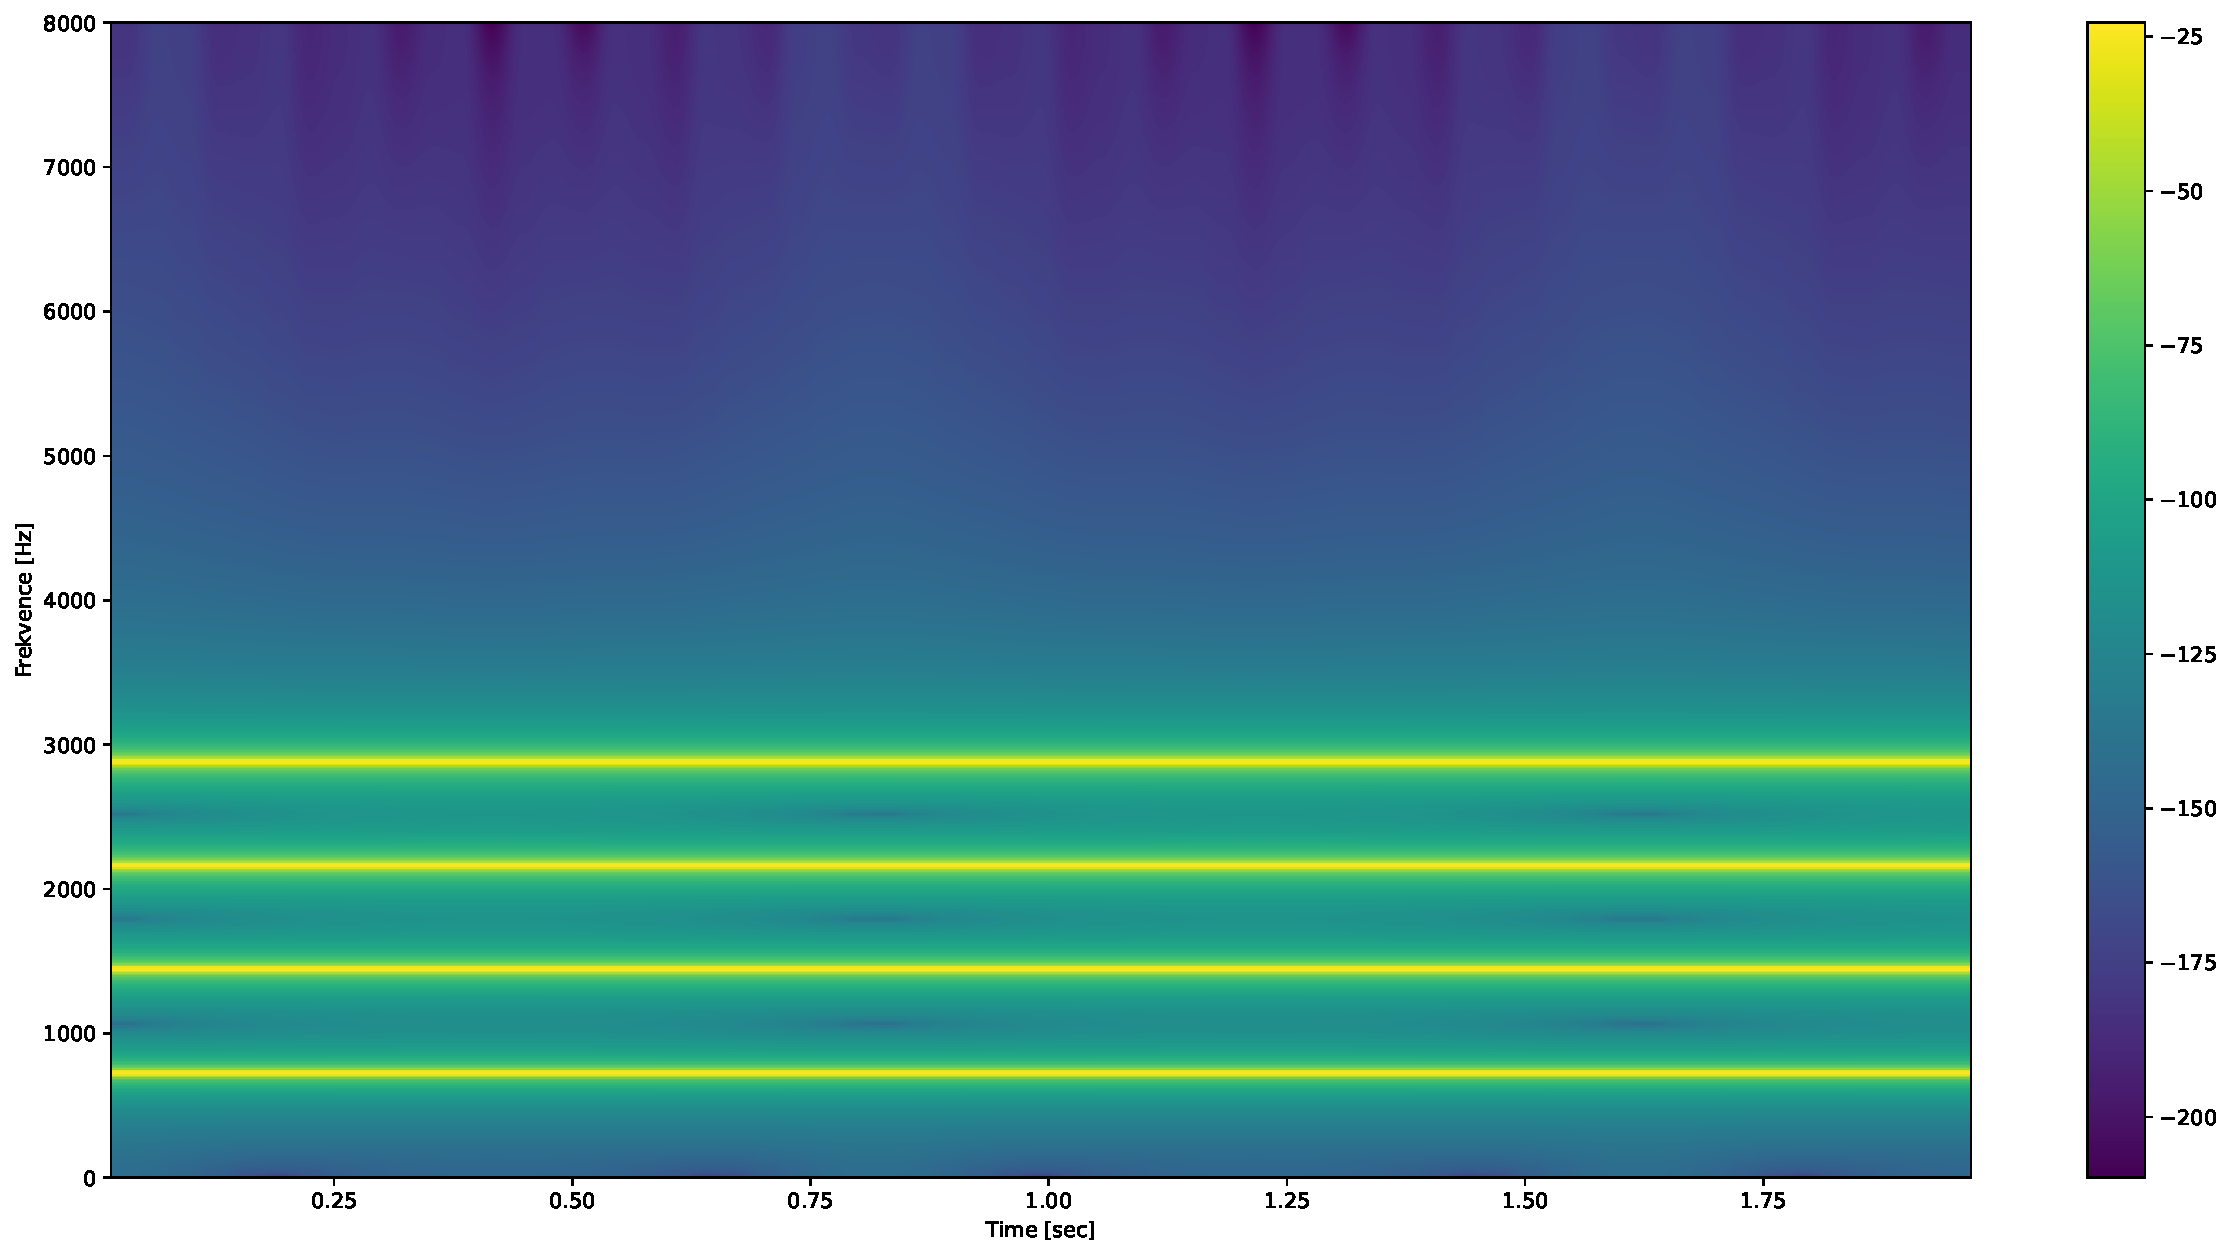
\includegraphics[scale=0.43]{img/4_4cos.pdf} \\
\end{center}

% ####################################################


% Generování signálu ##############################################
\newpage
\section{Čistící filtr}
\subsection{Výroba filtru v z-rovině}
Rozhodl jsem se vytvořit filtr signálu 1. návrhu ze zadání - Výroba filtru v z-rovině. Filtr dobře filtruje nežádoucí frekvence, které byly nalezeny v signálu. Filtr, také bohužel zkresluje signál, protože potlačuje veškeré frekvence v rušivém pásmu, což znehodnotí původní nahrávku, jelikož ta mohla mít frekvence v tomto pásmu také. Na následujícím obrázku je filtr vyjádřen pomocí impulzní odezvy:

\begin{center}
        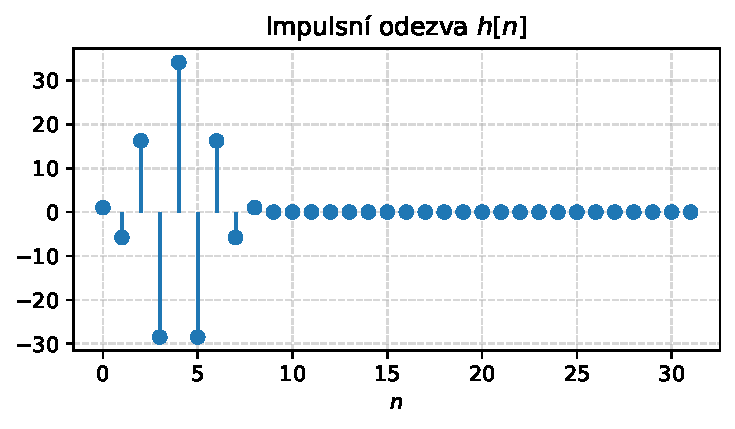
\includegraphics[scale=0.7]{img/5_filter_impuls.pdf} \\
\end{center}


Jelikož mám FIR filtr, tak jediný 'a' koeficient bude 1.  Koeficienty filtru zaokrouhlené na 2 desetinná místa jsou vidět v následujících tabulkách:

%
% 0 1.0
% 1 -5.783425536135367
% 2 16.216655472257226
% 3 -28.466669114134323
% 4 34.086112333566504
% 5 -28.466669114134323
% 6 16.216655472257226
% 7 -5.7834255361353675
% 8 1.0000000000000002

\begin{table}[ht]
    \centering
    \begin{tabular}{| c | c | c | c | c | c | c |  c |  c |}
    \hline
        b[0] & b[1] & b[2] & b[3] & b[4] & b[5] & b[6] & b[7] & b[8]  \\ \hline
        1 & -5.78  & 16.22 & -28.47 & 34.09 & -28.47 & 16.22 & -5.78 & 1   \\ \hline
    \end{tabular}
\end{table}

\begin{table}[ht]
    \centering
    \begin{tabular}{| c |}
    \hline
        a[0] \\ \hline
         1    \\ \hline
    \end{tabular}
\end{table}




Následující kód popisuje, jak jsem filtr implementoval v pythonu.
\begin{minted}{python}
    ## Vytvoření koeficientů filtru 'b' se doplní později
    a = [1, 0, 0, 0, 0, 0, 0, 0, 0, 0]  ## a y[n]
    b = []                              ## b x[n]
    
    # Spočítání nulových bodů, které budou tvořit koeficienty B.
    for i in range(1,5): # Pro rušivé frekvence (f_bad*1 - f_bad*4)
        wi = 2*np.pi*((f_bad*i)/sample_rate)  # převod na norm. kruh. frek.
        ni = np.e**(1j*wi) # Výpočet nulového bodu
        ni_k = np.conj(ni) # Výpočet komplexně sdruženého nulového bodu.

        b.append(ni)       # Připojí koeficienty do pole b
        b.append(ni_k)

    # Funkce, která jednotlivé koeficienty transformuje pro filtr,
    # jelikož to byla komplexní čísla a potřebujeme reálná.
    b = np.poly(b)         

    return a, b
\end{minted}

Pozn: Při implementaci charakteristiky filtru (jednotkový impuls, nuly a póly...) jsem se inspiroval v materiálech ing. Žmolikové.

% ####################################################


% Nulové body a póly ##############################################
\section{Nulové body a póly}
Zde jsou mé nulové body a póly. Pól mám jenom jeden v hodnotě [0,0], Našel jsem tedy jenom jeden bod, ve kterém je jmenovatel přenosové funkce roven 0, zatímco pólů je celkem 8 a všechny leží na kružnici.

\begin{center}
        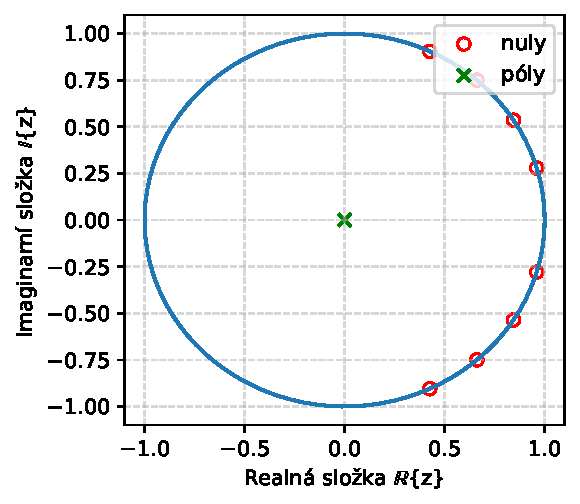
\includegraphics[scale=1]{img/9_np.pdf} \\
\end{center}



% ####################################################


% Frekvenční charakteristika ##############################################
\section{Frekvenční charakteristika}
Jelikož jsem nedělal filtr pro každou nežádoucí frekvenci zvlášť, ale udělal jsem filtr, který potlačuje více nežádoucích frekvencí najednou, tak jde vidět jistý špatný trend. Nejen, že filtr potlačuje frekvence 720Hz 1440Hz, ale i blízké okolí těchto frekvencí, což znehodnocuje původní signál. \\
% ####################################################
\begin{center}
        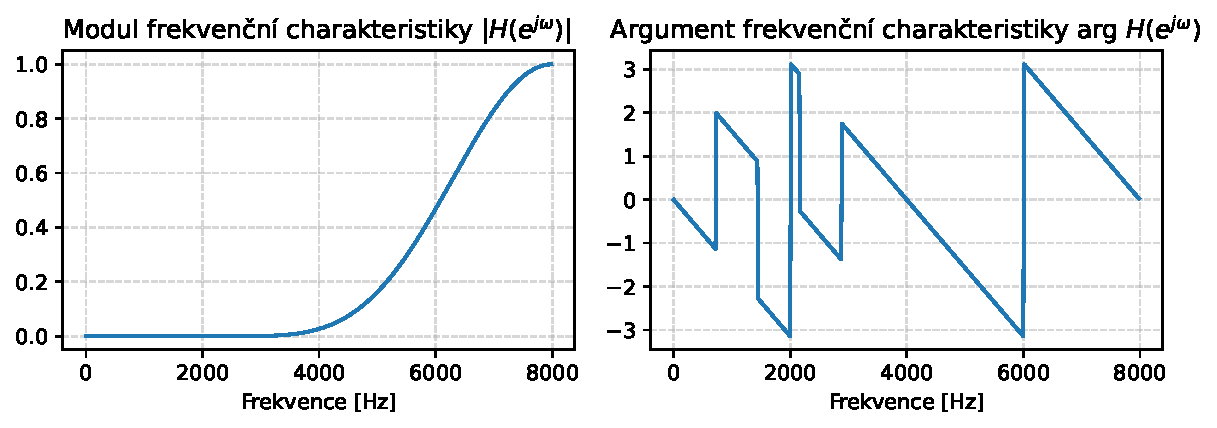
\includegraphics[scale=0.85]{img/6_freq_char.pdf} \\
\end{center}


% Filtrace ##############################################
\newpage
\section{Filtrace} 
Tady mám výsledný vyfiltrovaný signál původní nahrávky, který je normovaný. A spektrum tohoto signálu, kde jde hezky vidět, že jsme se zbavil původních nežádoucích horizontálních čar, ale zanechalo to stopu. Poslechem lze poznat, že se signál zbavil nepříjemného pištění a je srozumitelnější. Výsledek však zdaleka není dokonalý a stále tam je rušivé šumění. Graficky jde velmi dobře vidět, že se signál zbavil tlusté čáry kolem středu, což byly výše zmíněné rušivé frekvence.\\

Filtrovaný signál:
\begin{center}
        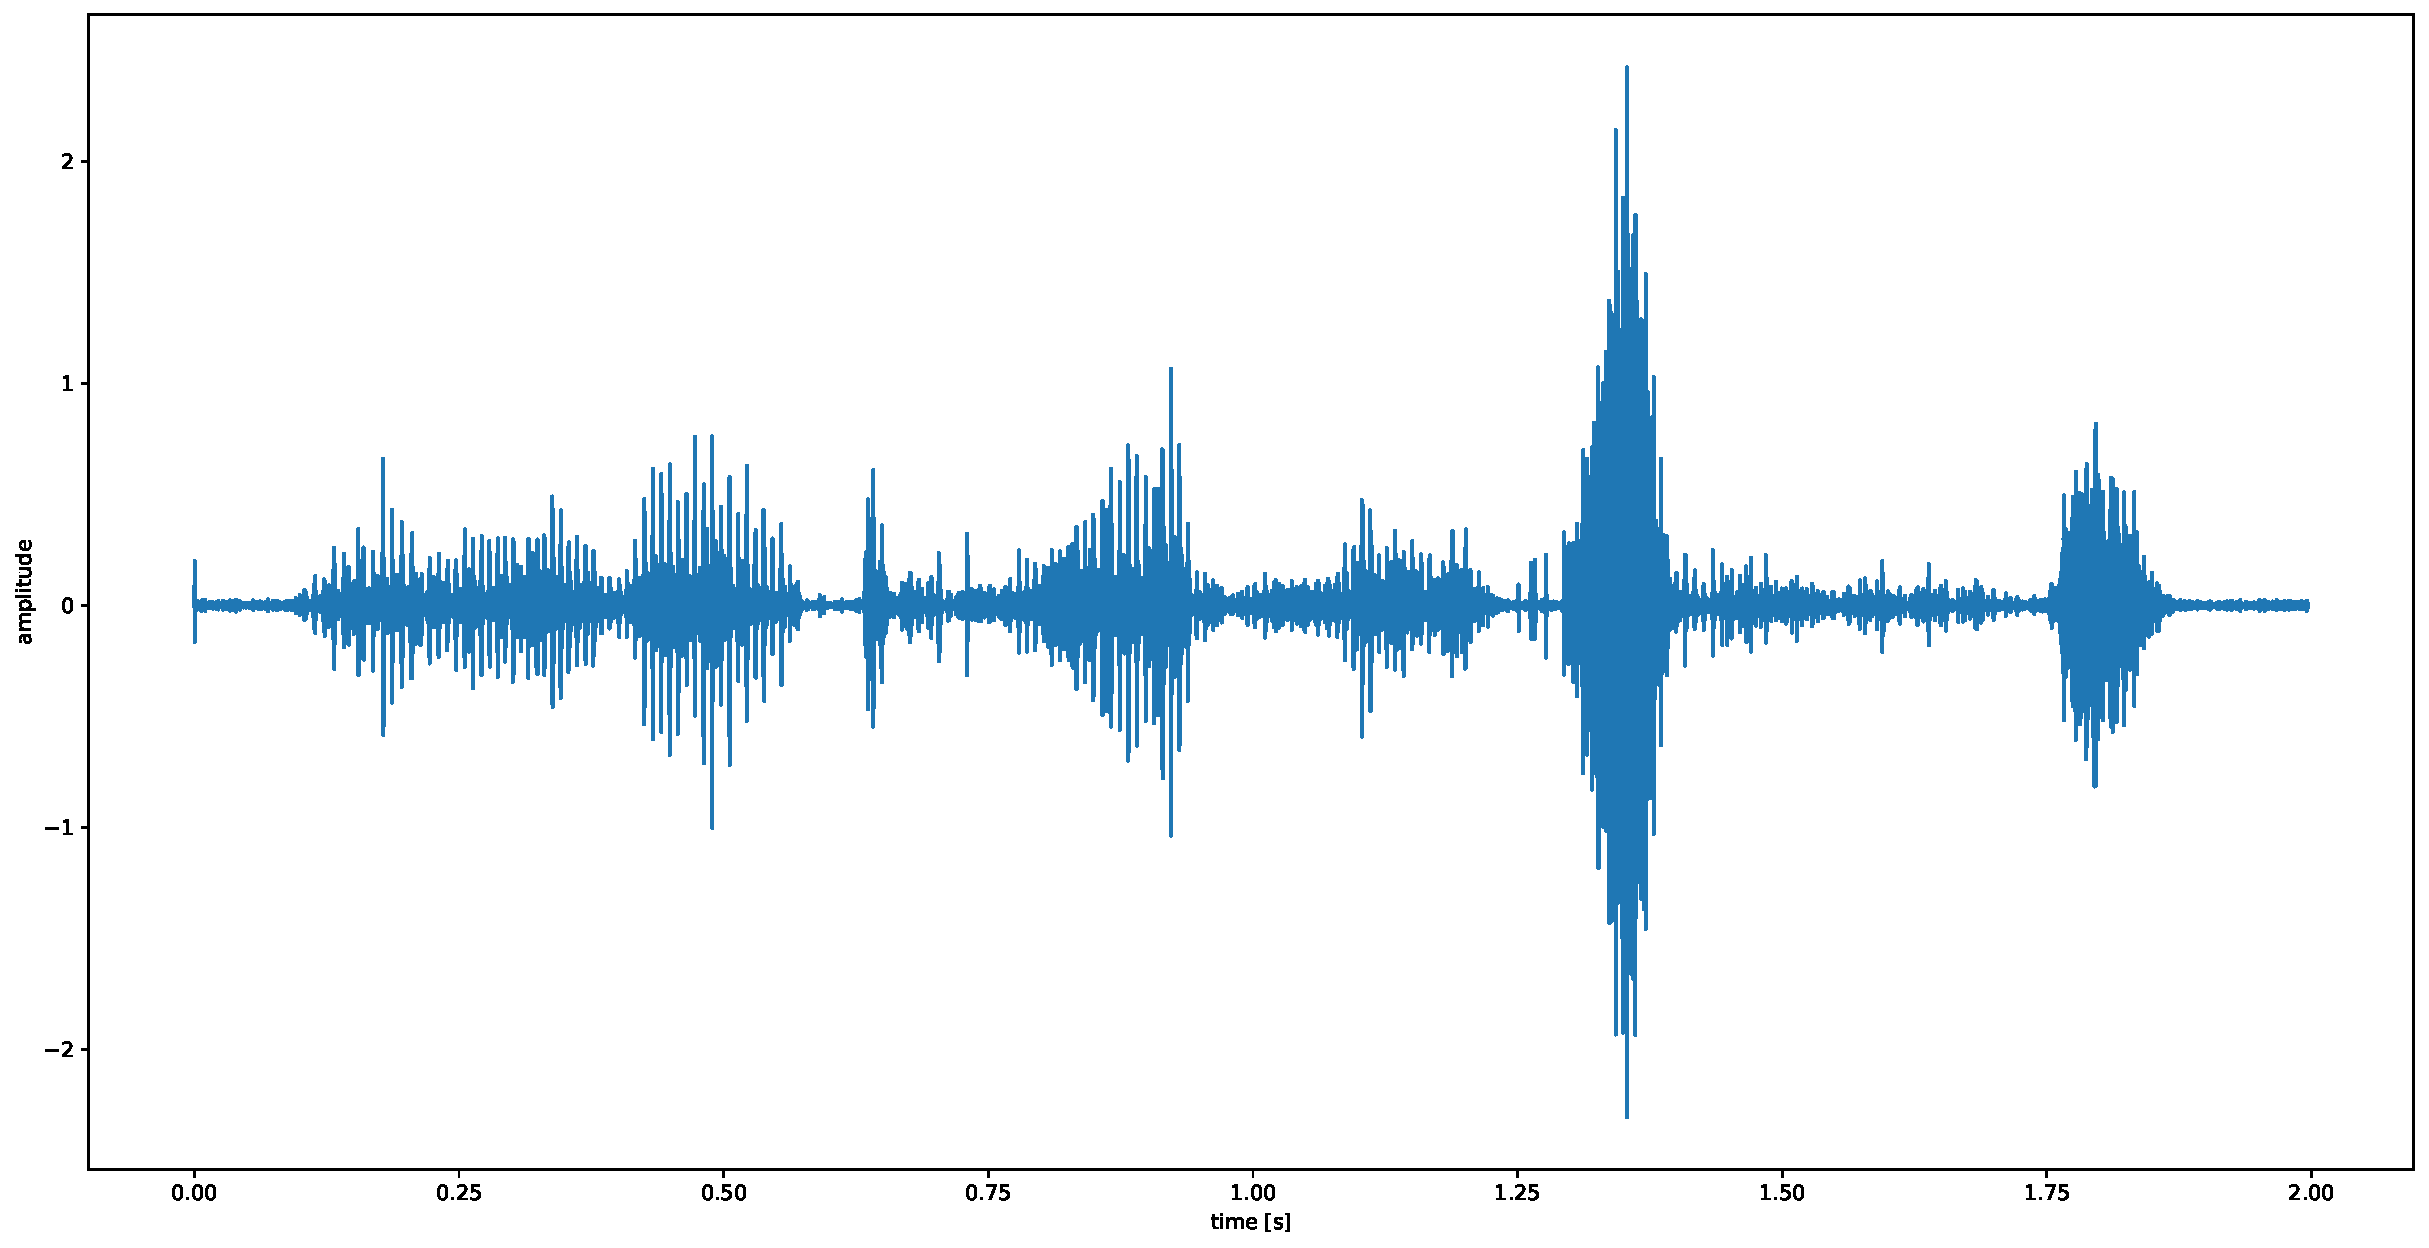
\includegraphics[scale=0.4]{img/8_filtered.pdf} \\
\end{center} 
Spektrogram filtrovaného signálu:
\begin{center}
        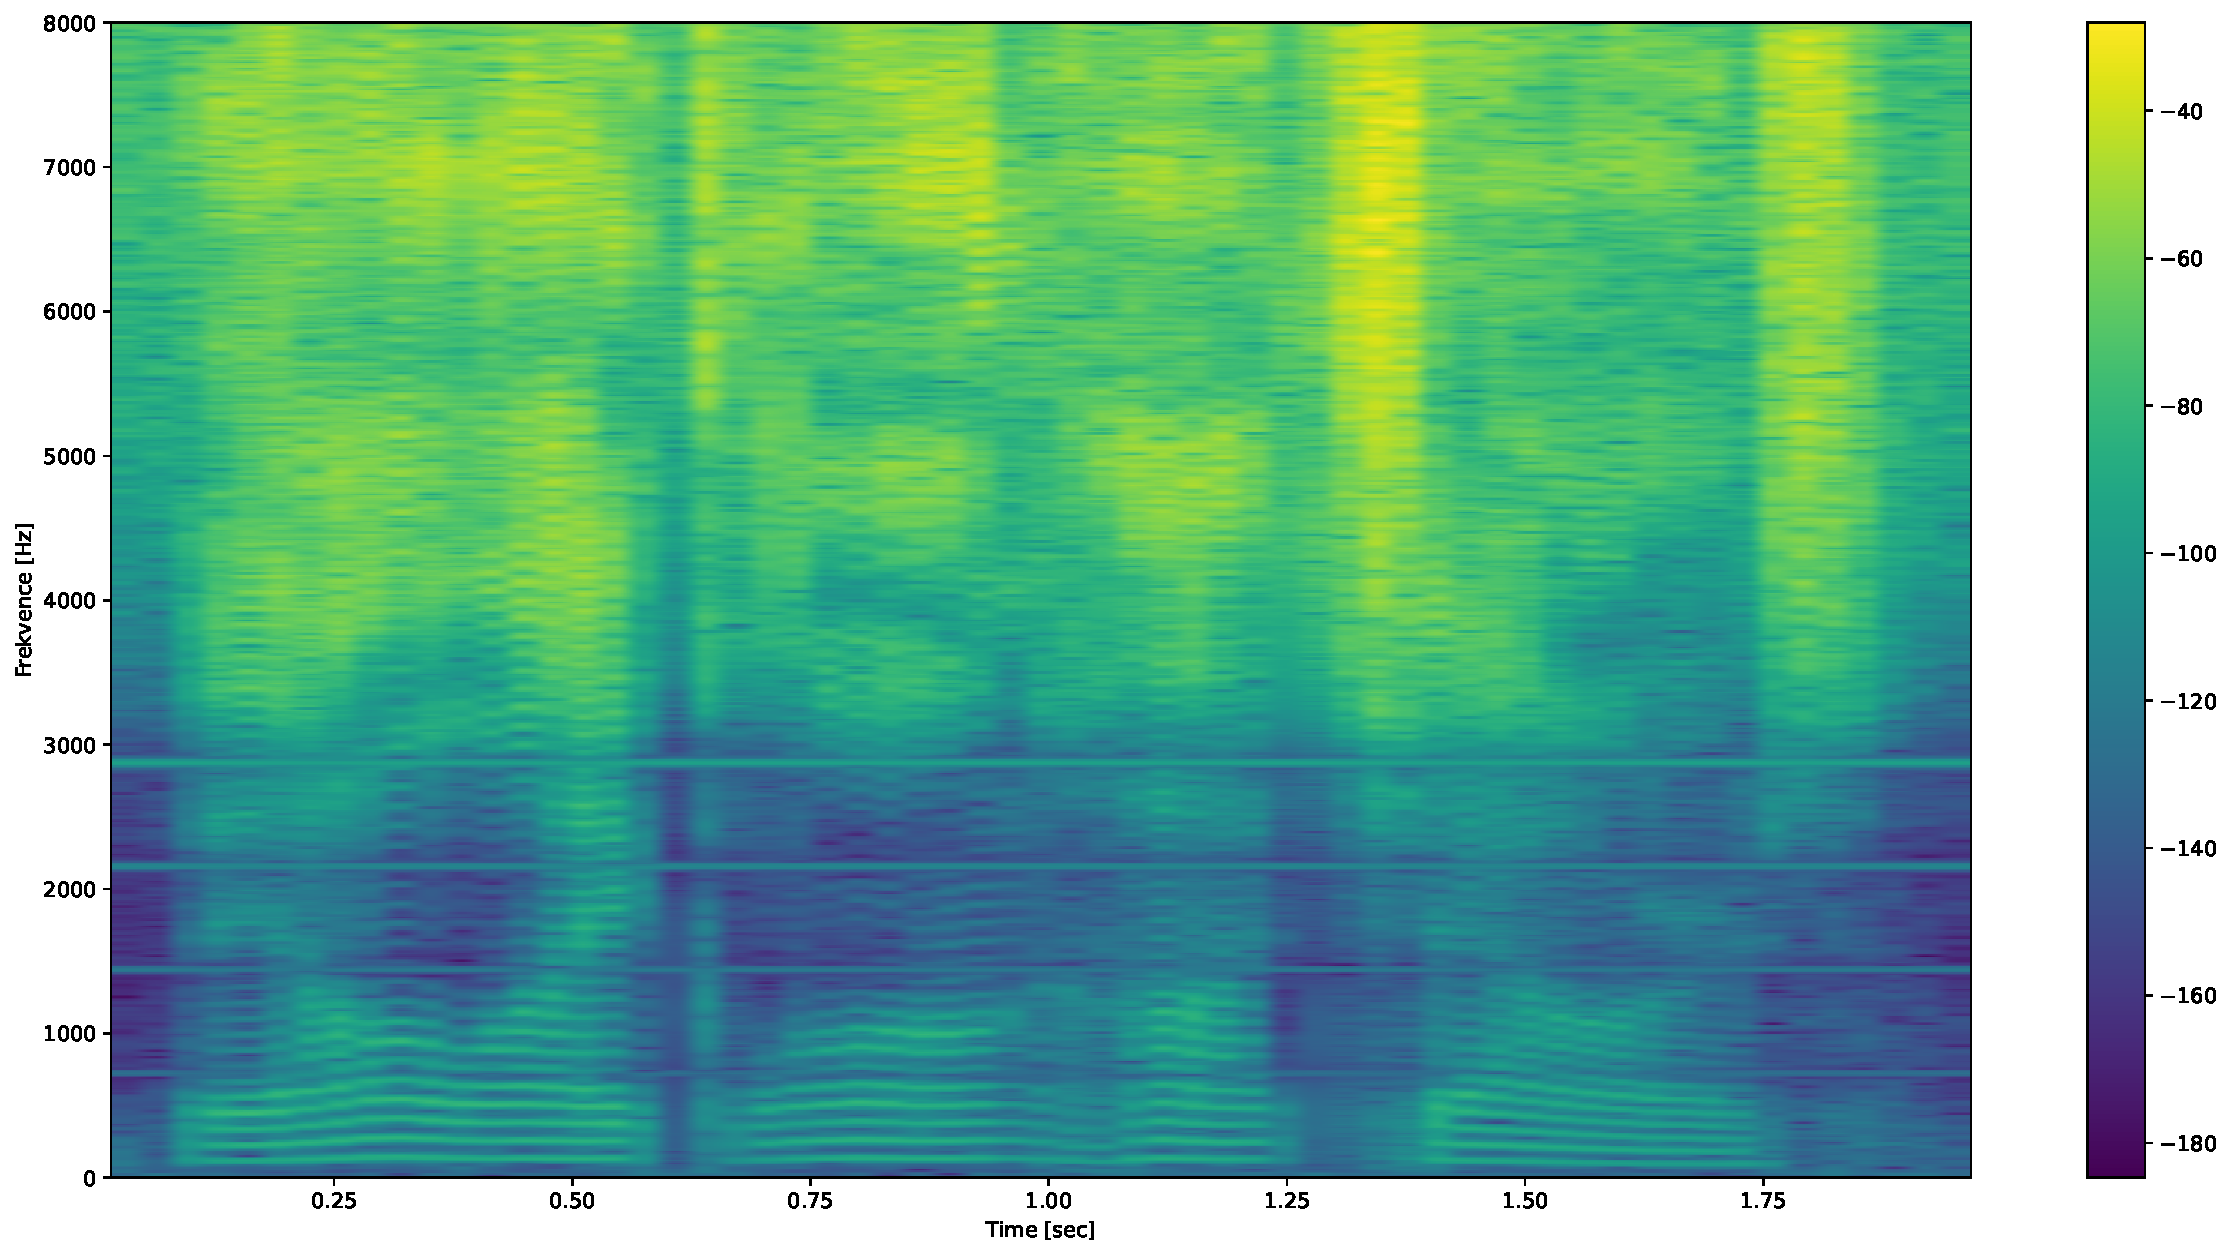
\includegraphics[scale=0.45]{img/7_filtered_spec.pdf} \\
\end{center}

% ####################################################





\newpage
\section{Zdroje}
práce s numpy: https://naucse.python.cz/lessons/intro/numpy/ \\
Vygenerování obrázku ze signálu: https://docs.scipy.org/doc/scipy/reference/generated/scipy.io.wavfile.read.html \\
dft vysvětlení: https://www.youtube.com/watch?v=nl9TZanwbBk \\
dft implementace http://blog.o1iver.net/2011/12/06/python-discrete-fourier-transformation.html \\
FILTRY: https://nbviewer.org/github/zmolikova/ISS\_project\_study\_phase/blob/master/Zvuk\_spektra\_filtrace.ipynb

\end{document}